\chapter{The low back vowels}
\label{ch:low_back}

\section{Introduction}

A study of the Elsewhere Shift would not be complete without at least a cursory look at the low back merger. The merger of \lot and \thought is claimed to be the trigger for the Elsewhere Shift, because \trap moves into the space previously occupied by \lot (see \S\ref{sec:structure_of_elsewhere_shift}). The retraction (and possibly raising) of the now-merged low back vowel leaves more room for this retraction to occur.

Previous work on nearby areas coupled with the findings from the previous two chapters lead me to the hypothesis that the low back vowels are merged and have been for some time in Cowlitz County. Though some areas of the West report an incomplete merger (\S\ref{sec:structure_of_elsewhere_shift}), in Oregon and elsewhere in Washington, the low back merger is reported to have been completed for several generations already \citep{mclarty_etal_2016, wassink_2016_pads}. Given that Cowlitz County is sandwiched between these two areas, it would only make sense to find a similar pattern here. Furthermore, because \bat-shifting has been present in this community since as early as 1930 (\S\ref{sec:what_kind_of_shift}), the low back merger should theoretically be found in all generations as well, assuming it acts as the trigger for \bat movement.

Nevertheless, the results in this chapter go contrary to my expectations.\footnote{It was not my original intention to include an analysis of the low back merger in this dissertation, but the patterns shown here and the shifts reported in other chapters warranted its inclusion to paint a more complete picture of this shift.} Even though Cowlitz County is in the middle of two areas with complete and stable mergers, and even though \bat has been shifting for several generations, which might suggest it was triggered by the low back merger before that, this chapter reports that the low back merger is, in fact, not a part of the speech of this community. The relative timing of the merger and \bat-retraction has implications for the Elsewhere Shift and whether the merger is structurally related to (and indeed, the trigger of) the lowering and retraction of the front lax vowels. This chapter sheds some light on the mechanisms of these changes in Cowlitz County.


\section{Methods for the study of merger}
\label{low_back_merger_methods}

The first thing to establish is whether the low back vowels are merged in Cowlitz County. So far in this dissertation, I have treated vowels independently and have not approached the topic of merger. Since this is the only chapter where merger is discussed, and because the classification of the \lot and \thought vowels can be problematic, it is requisite to discuss some of the methods used here.

\subsection{Defining \lot and \thought}

In \S\ref{corpus_size_constitution}, I explain that I manually corrected some of the other vowel classes in this study. This was necessary because the dictionary used by the Montreal Forced Aligner appears to have a few errors. This manual correction is especially important when studying a merger such as the low back merger. If the words are classified into incorrect categories, the two classes may appear to be closer together than they really are and an analysis may overestimate the degree of merger. Conversely, \citet[39]{strelluf_2019} points out that if the dictionary contains multiple entries for a single word, it may artificially separate the two classes in speakers with the merger.

To my knowledge, there is not a clear consensus regarding which words belong to which categories. By this I mean there is no easily accessible database, one that has been verified by speakers without the merger, that shows the complete \lot and \thought lexical sets. In fact, such a list would be problematic in and of itself because of idiosyncratic variation vowel categorization. Furthermore, \citet{dinkin_2016} points out that some speakers have the merger in some phonological contexts, such as before coda laterals but not intervocalic laterals.\footnote{Speakers who have this particular merger---like me---would pronounce words that historically contain the \lot vowel, like (\textit{doll}, \textit{golf}, \textit{revolve}, and \textit{volcano}) with the backer \thought vowel so that they sound like \textit{all}, \textit{small}, or \textit{hall}. However, they would continue to use the fronter vowel in words like \textit{dollar}, \textit{holly}, \textit{college}, \textit{solid}, and \textit{psychology}, such that \textit{collar} and \textit{caller} form minimal pairs.}

Nevertheless, the words do need to be classified in some way to make comparisons. \citet[133]{hall_lew_2009_diss} explains that because she has the merger in her own speech, she classified her tokens into \lot and \thought based on lists presented in previous studies. For words that were in her corpus but not classified in a previous study, she asked sociophoneticians who do not have the merger for their intuitions and coded them based on their consensus. Similar methods were adopted by \citet[note 4]{podesva_etal_2015}. Since I retain a relatively clear distinction between \lot and \thought in most environments,\footnote{I was born and raised in O'Fallon, Missouri and lived there until I was 18. My father lived in Upstate New York until he was 12 when he moved to Minnesota. My mother grew up in Minnesota. In casual measurements of my own pronunciation, my vowels are distinct except before tautosyllabic /\textipa{l}/ and sometimes before nasals and /\textipa{g}/.} I classified each word as either belonging to \lot or \thought based on my own intuition.

This imposition of my speech patterns onto the data is admittedly an unscientific approach, but the fact that the LibriSpeech corpus transcribed \textit{lot} with \thought and \textit{thought} with \lot---the very words the word lexical sets are named for!---meant that some adjusting had to be done. Some of the discrepancies between my classification and the LibriSpeech corpus transcriptions were based on historical groupings. For example, several words were transcribed with \lot but are spelled with $<$au$>$ or $<$aw$>$ (\textit{auction}, \textit{audio}, \textit{audit}, \textit{August}, \textit{awful}, \textit{bought}, \textit{caught}, \textit{cause}, \textit{law}, \textit{raw}, etc.) and were switched because this spelling corresponds to Middle English /au/ and these words historically belong to \thought \citep[115]{wells_1982}. But comparing my intuitions with the sets that \citet[133--134]{hall_lew_2009_diss} lists, there are a few differences. For example, I classified \textit{Broncos} and \textit{stomping} as part of \thought and some words like \textit{probably}, \textit{mom}, \textit{pond}, and \textit{prom} are admittedly difficult to classify and could go either way. Two of these words, \textit{probably} and \textit{mom} are especially problematic for this study because they are among the most common words that contain either of the low back vowels. Therefore, in cases where my intuition does not match the classification in \citet[133--134]{hall_lew_2009_diss}, I used Hall-Lew's classifications in this study.\footnote{As it turns out, in a previous analysis I classified \textit{probably} and \textit{mom} into \thought based on my own speech and it did in fact create an artificially large distinction. In that previous analysis, the difference between the two vowels was quite larger than what is now reported in this section. So even small adjustments to the vowel categories can have substantial effects on the overall results.} Not only is her list a consensus based on several other sociophoneticians' intuitions, it makes the methods in this study a little more objective and more in line with other studies in the West. The complete set of \lot and \thought words in this study is listed in Appendix \ref{appendix:lowback_categories}.

Finally, tokens where the vowel is followed by a lateral or rhotic are excluded from analysis. This makes the analysis of \lot and \thought more comparable to the analysis of \trap, \dress, and \kit in this study, and eliminates the potential problem of imposing my partial merger before liquids.


\subsection{Using GAMMS to study vowel merger}

With these classifications set, a generalized additive mixed-effects model was fit to all tokens of \lot and \thought pooled together. While previous models included a three-way interaction term---one that combined sex, generation, and formant---as the primary predictor, this model instead used a four-way interaction term that combined those three predictors with vowel class. Thus, this categorical variable included 32 different levels (all combinations of the two sexes, four generations, two formants, and two vowel classes) which were all treated independently. As with the other models, this variable was included as a parametric effect and as a smooth.

Other than the addition of vowel in the model specification, the analysis of merger using GAMMs is similar to how shifting is measured in previous chapters: by way of visualizations of predicted measurements, model summaries, model comparison, and difference smooths.\footnote{See Appendix \ref{appendix:difference_smooths} for a primer on how to interpret difference smooths.} In particular, the difference smooths allow the researcher to identify not only if the vowels are significantly different from one another, but where along the trajectory of the vowel this difference may be. Using vowel trajectories to study vowel merger is not new in the Pacific Northwest (see \citealt{freeman_2014}), but to my knowledge using GAMMs and difference smooths to do so is.

\section{The low back merger}
\label{low_back_merger}

Figure \ref{fig:bot_and_bought} show the average trajectories for \lot and \thought in the four generations by sex. These patterns have been presented indirectly already in many of plots in previous chapters as light gray lines when vowels are shown in the context of the full vowel space. But in Figure \ref{fig:bot_and_bought}, we see clearly that the two vowels are different. Not only is \lot a fronter and lower vowel (reflecting its historical distribution), but \thought has a somewhat of a wider trajectory and passes through more of the F2 space than \lot does. In other words, \thought has more of a U-shaped pattern while \lot is ``pointier.''

\begin{figure*}[tb!]
    \centering
    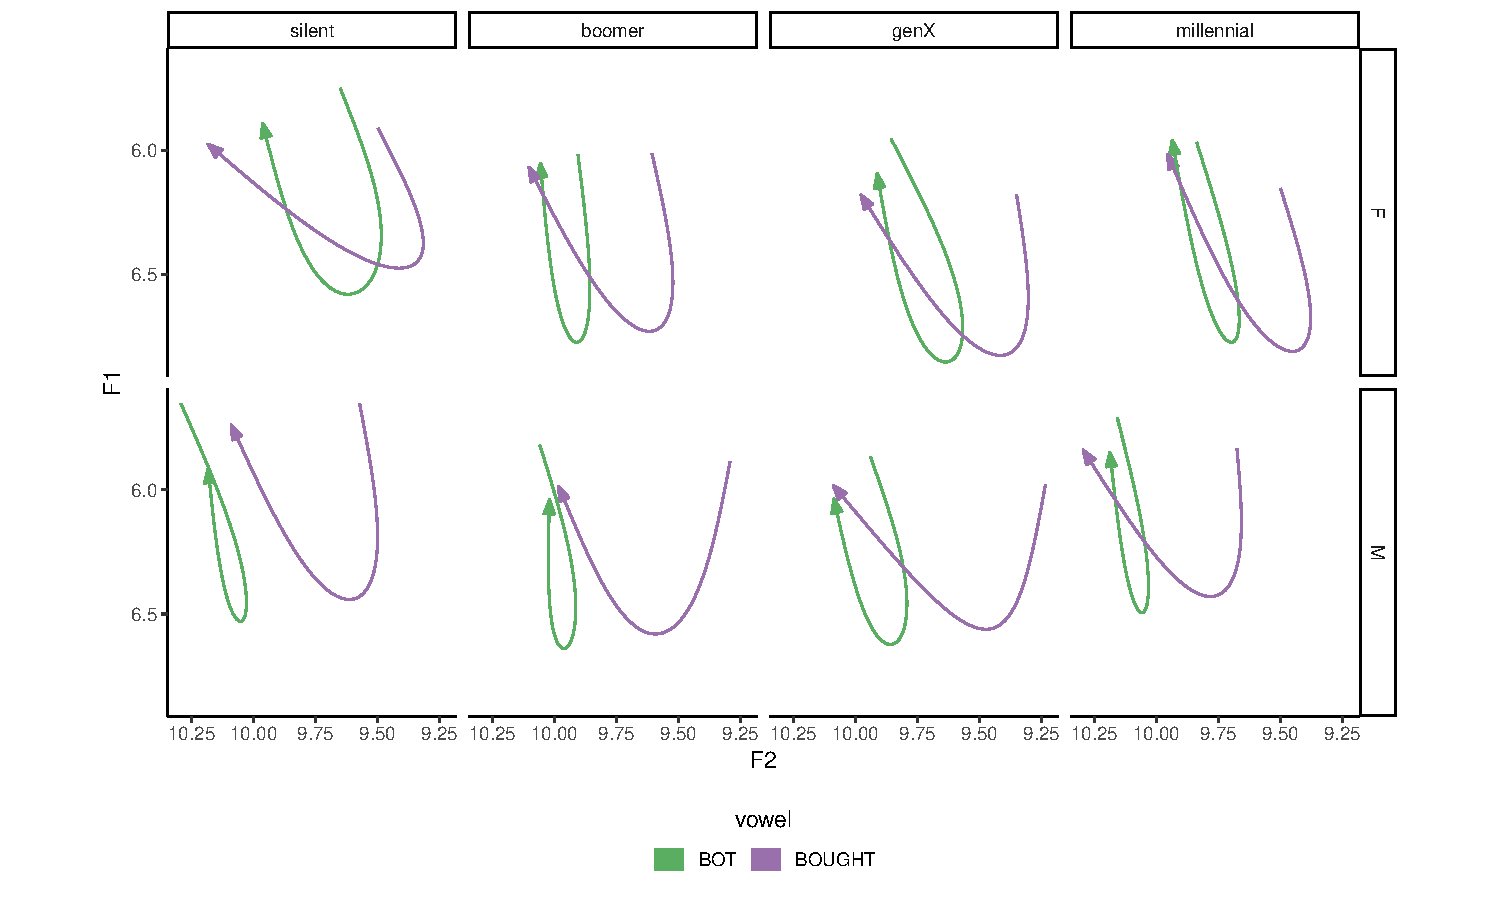
\includegraphics[width = 6.5in]{Figures/other_figures/low_back_trajs.pdf}
    \caption{\lot and \thought by sex in four generations.}
    \label{fig:bot_and_bought}
\end{figure*}

The two trajectories do share some similarities. In terms of formant movement, F1 rises and falls like most other vowels in this study and F2 either raises slightly to peak somewhere in the first half of the trajectory, or it increases throughout the duration of the vowel.

These trajectories resemble descriptions of the low back vowels in other communities. For example, in St. Louis, \citet[176]{majors_2005} finds that speakers raise and then lower F1 and that their F2 movement in \thought is much greater than for \lot. \citet[159--161]{irons_2007} also finds that \thought's trajectory length was longer in some Kentucky speakers. So, in Cowlitz County, while \thought continues to be the more dynamic vowel, it lacks the high onset found in other communities.

Another similarity shared between these two vowels is that their target, which is the point when and where F1 reaches its peak, is approximately the same for all groups of people. All 16 trajectories presented in Figure \ref{fig:bot_and_bought} had a peak F1 between 48\% and 57\% into the duration of the vowel. More importantly for the merger, the position in the F1-F2 space at that target was very similar for all groups. In other words, the midpoints are all quite similar---it is the trajectories that are distinguishing these vowels. If only the midpoints were sampled, these speakers would indeed exhibit a high degree of overlap between these two vowels and one would conclude that they are indistinguishable. But because trajectory information is included, systematic differences between the vowels are found.

\begin{figure*}[p]
    \centering
    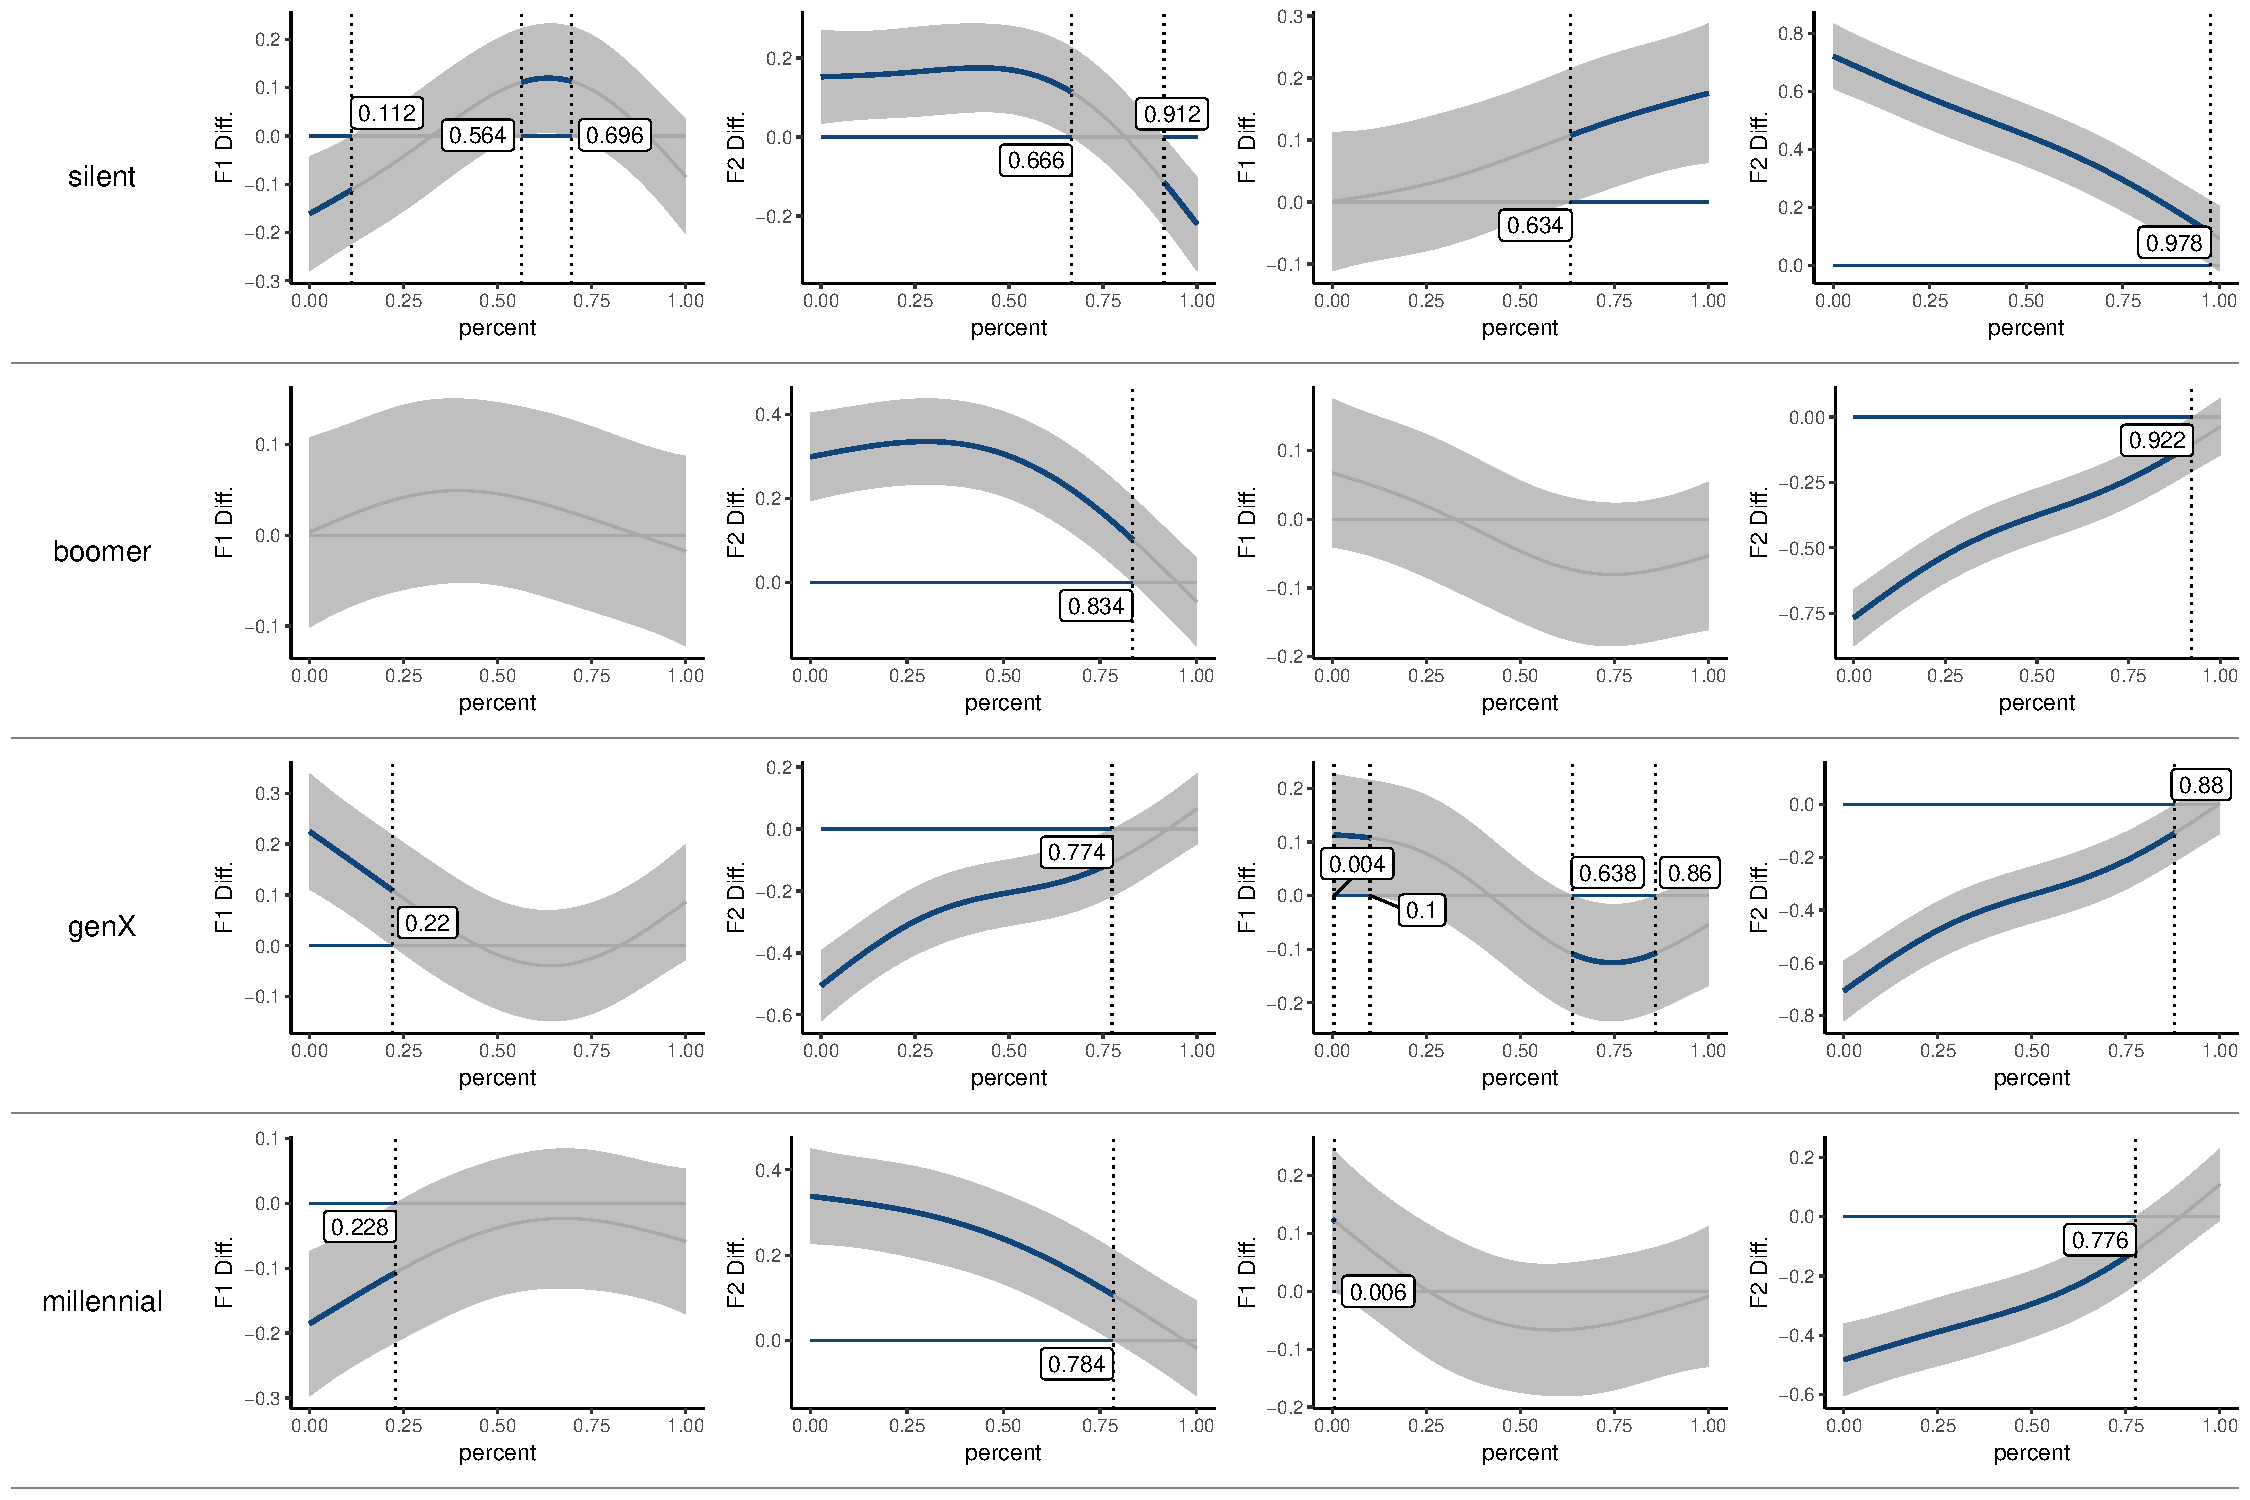
\includegraphics[angle=90, origin=c, height = 6.5in]{Figures/other_figures/low_back_diff_smooths.pdf}
    \caption[Difference smooths for the low back vowels]{Difference smooths for the low back vowels by generation, sex, and formant. Rows represent generations. The columns are F1 women, F2 women, F1 men, F2 men.}
    \label{fig:low_back_difference_smooths}
\end{figure*}

To illustrate that these two vowels are indeed different, Figure \ref{fig:low_back_difference_smooths} shows the difference smooths, comparing the two vowels by formant, sex, and generation. In previous chapters, these difference smooths were relegated to Appendix \ref{appendix:difference_smooths} because of space issues, but because establishing whether \lot and \thought are merged is a crucial element in this analysis, I present the full grid of plots here.

The patterns shown in these difference smooths are somewhat more complex than what has been presented for the other vowels, particularly in F1. Beginning with the women (the two columns on the left when the page is rotated), we see that the difference between the two vowels is significant for small portions of F1, somewhat haphazardly across generations. For three of the generations, it was primarily during the onset of the vowel that the distinction was found. However, for F2, the two vowels were kept distinct for at least three quarters of the duration of the vowel, chiefly the first three quarters. In other words, the two vowels start off in different places, but they end in the same place. In the men, there were some windows where the vowel height difference was significant, but there are no obvious patterns. In F2, however, the men are like the women, where \thought is significantly further back than \lot for the majority of the vowel space. In fact, the men keep this distinction for nearly the entire length of the vowel. The common pattern in both sexes is that speakers in Cowlitz County do not appear to have a robust height difference between the two vowels\footnote{I have chosen my words carefully here. It is somewhat nonsensical to claim that \lot and \thought are ``merged'' in F1 because, after all, so are \fleece and \goose. A high degree of overlap in one formant alone says little about the status of merger between those two vowels.} and that they retain and F2 difference between \lot and \thought.\footnote{This F2 distinction between \lot and \thought is far bigger than the difference between two generations' realizations of the same vowel. The width of the confidence intervals in the F2 columns appears so much narrower than in any of the other figures because the \textit{y}-axis covers a much wider range (or rather, the plot had to be zoomed out to accommodate the wide gap) than any of the difference smooths in the appendix.}

\begin{figure*}[tb!]
    \centering
    \hspace{\fill}
     \begin{subfigure}[t]{2.925in}
        \centering
        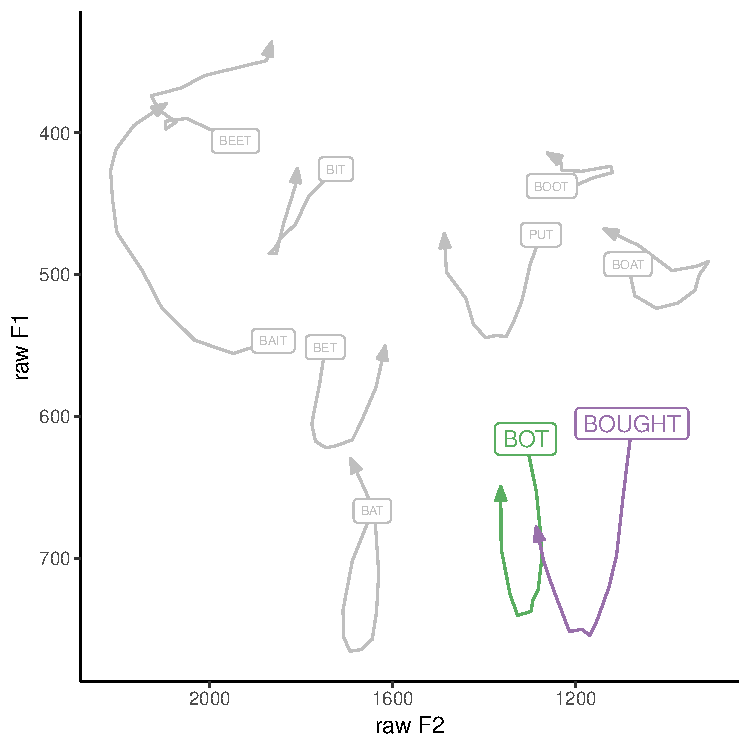
\includegraphics[width = \textwidth]{Figures/example_plots/09-Dale_avg_lowback.pdf}
        \caption{Dale's low back vowels.}
        \label{fig:dale_low_back}
    \end{subfigure}
    \hspace{\fill}
    \begin{subfigure}[t]{2.925in}
        \centering
        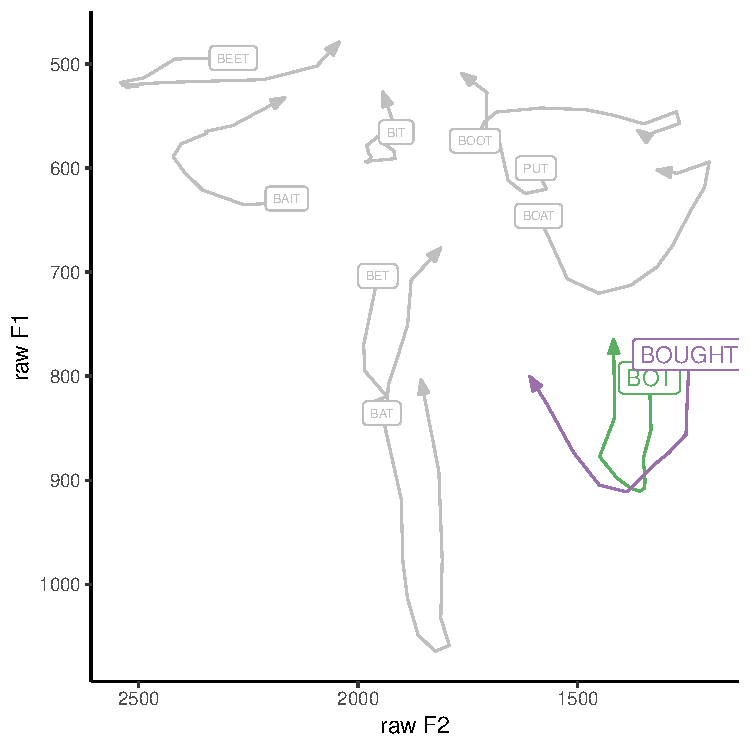
\includegraphics[width = \textwidth]{Figures/example_plots/14-Jessica_avg_lowback.pdf}
        \caption{Jessica's low back vowels.}
        \label{fig:jessica_low_back}
    \end{subfigure}
    \hspace{\fill}
    \caption{Sample plots showing a separation between the low back vowel.}
    \label{fig:dale_and_jessica}
\end{figure*}

That these vowels are distinguished holds true when examining individuals' average vowel trajectories. Figure \ref{fig:dale_low_back} shows the vowels of Dale, a man born in 1936, and Figure \ref{fig:jessica_low_back} presents the vowels of Dale's granddaughter, Jessica, who was born in 1998. Dale's low back vowels are similar in their trajectory and overall height, but the primary factor distinguishing them is F2. As a male from the Silent Generation, Dale represents what is usually the most linguistically conservative group of speakers in a given community. His speech exhibits characteristics of other more conservative features such as \goose and \goat being relatively back and monophthongal, and little shifting and lowering of the front lax vowels. His low vowels are different, but are admittedly closer together than any other pair of vowels.

Conversely, Jessica, a female Millennial\footnote{Actually, Jessica is technically in Generation Z because she was born after 1997!} exhibits many innovative Washington features, such as a more monophthongal \face, fronted and diphthongal back vowels, and retracted front lax vowels, including a remarkably low and diphthongal \bat. Nevertheless, Jessica lacks what is perhaps the most characteristic feature of Western American English: the low back merger. Of her two low back vowels, Jessica's \thought has a more dynamic trajectory, starting further back than \lot, passing it near the midpoint, and ending up more centralized. The two have nearly identical midpoint measurements, but are kept distinct by their trajectories. Her low back vowels are closer than her grandfather's, but are not merged.

To summarize this section, it appears that the low back merger is \textit{not} widespread in Cowlitz County. By itself, this not an unusual finding for a community in the West. But because the front lax vowels are indeed shifting in this community, the claim that \bat retracts as a result of the low back merger is not supported by this data. In the following sections, I provide a more complete account of each of the low back vowels in Cowlitz County, akin to what was done in the previous two chapters, and then conclude this chapter with some implications given the patterns in this data.






\section{\lot}
\label{BOT}

In this corpus, there were 6,370 tokens of \lot coming from 604 unique words. The most common of these words were \textit{got}, \textit{lot(s)}, \textit{mom}, \textit{probably}, \textit{job}, \textit{rock}, \textit{gotta}, \textit{top}, \textit{stop}, and \textit{gosh}. There was an average of 118 tokens per speaker\footnote{Speakers ranged from 58 to 210 tokens with a standard deviation of 34.8: 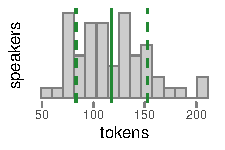
\includegraphics[width = 1.5in]{Figures/BOT/BOT_tiny.pdf}} and 796 per generation per sex.

%\begin{figure}[htb]
%	\centering
%	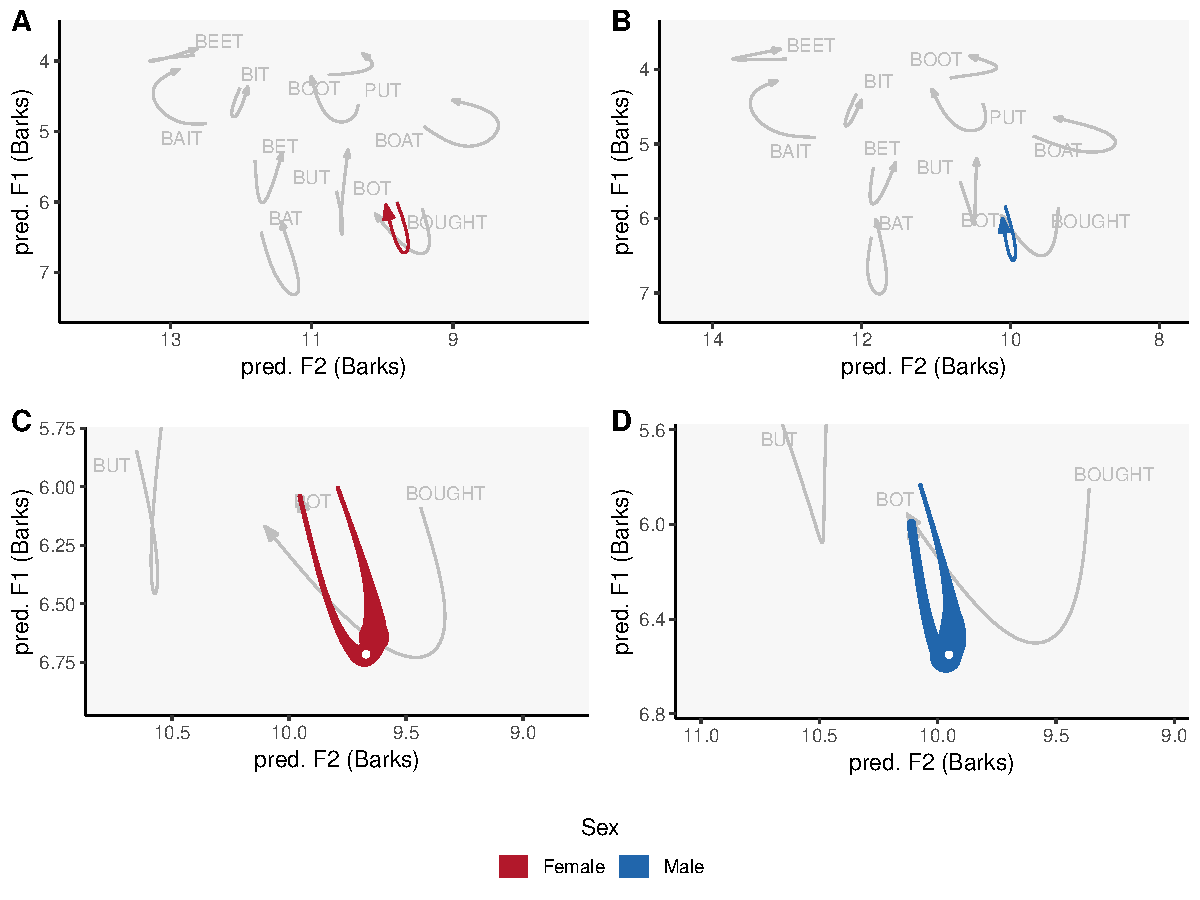
\includegraphics[width = \textwidth]{Figures/BOT/BOT_four_panel_plot_summarized.pdf}
%	\caption[Predicted formant measurements for \lot by sex.]{Predicted formant measurements for \lot by sex with women on the left and men on the right. Predicted values are averaged across all generations.}
%	\label{fig:BOT_four_panel_summarized}
%\end{figure}

%Figure \ref{fig:BOT_four_panel_summarized} shows the overall look at \lot in this community. As described previously, it exhibits a ``bounce''-like trajectory, with a rising-falling F1 which peaks very near the midpoint while keeping F2 relatively stable. \lot is also somewhat more fronted than \thought, especially for the men.

\begin{figure*}[tb!]
	\centering
	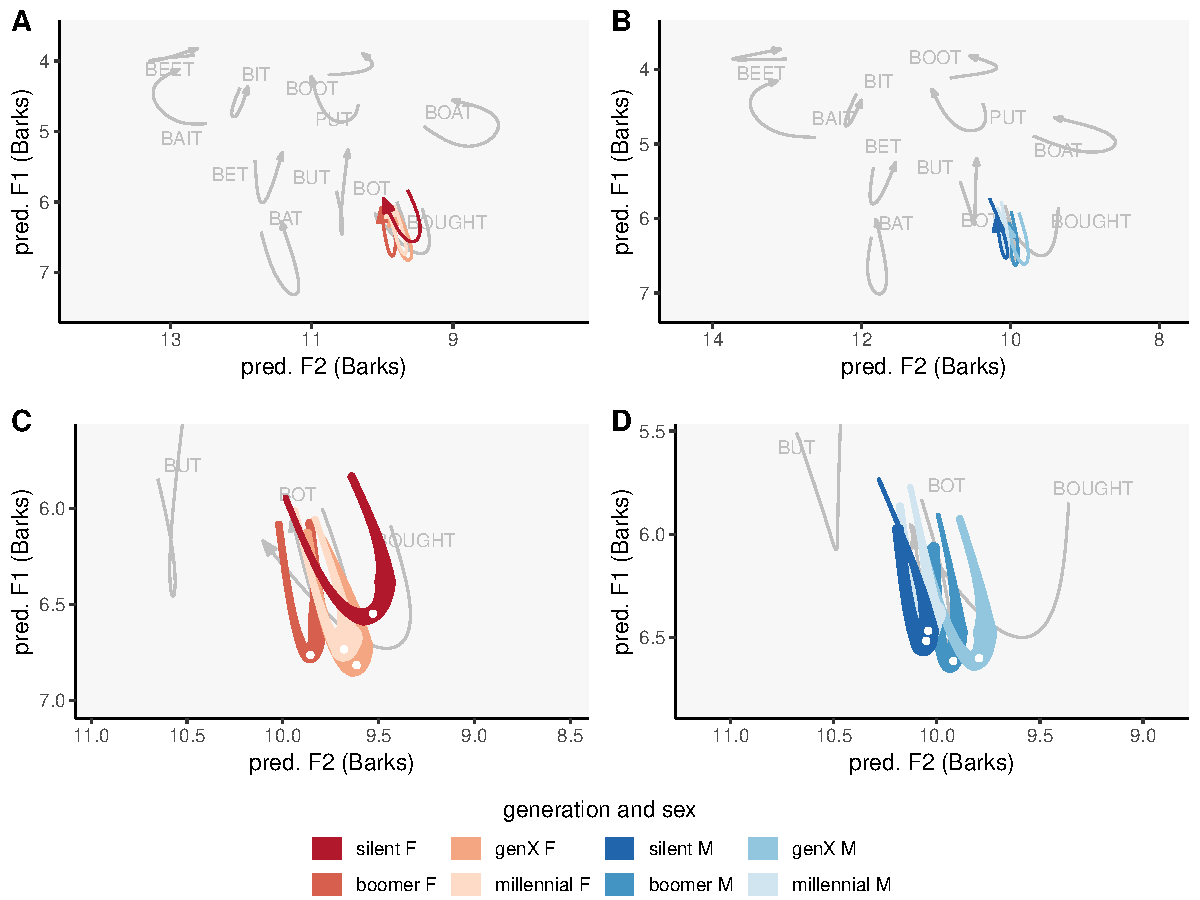
\includegraphics[width = 6.5in]{Figures/BOT/BOT_four_panel_plot.pdf}
	\caption[Predicted formant measurements for \lot by sex and generation.]{Predicted formant measurements for \lot by sex and generation. Women are on the left and men on the right. Darker shades represent older generations.}
	\label{fig:BOT_four_panel}
\end{figure*}

Though these trajectories have been shown already in Figure \ref{fig:bot_and_bought}, Figure \ref{fig:BOT_four_panel} groups them by sex to facilitate change in apparent time (as well as incorporating spectral rate of change via line thickness). In other western communities, the merged low back vowel is raising and retracting in the vowel space, so I expected to find that pattern here. This figure suggests no such raising or retraction; in fact, the difference between generations was small and somewhat haphazard.

Difference smooths suggest only a few minor shifts from one generation to the next. The Silent women were significantly higher and backer for some of the duration of the vowel than the Baby Boomers (\ref{fig:bot_diff_smooths_gen}A--B), which is actually opposite of the expected direction of change. There is even less change among the men, the largest difference being between the Silent generation and Generation X at the onset (\ref{fig:bot_diff_smooths_gen}D--H). For both sexes, the difference between Generation X and the Millennials was not significant (\ref{fig:bot_diff_smooths_gen}U--X), suggesting that whatever change there may have been in Cowlitz County with \lot, if there even was one, is no longer in progress.

The main takeaway from Figure \ref{fig:BOT_four_panel} is that there is very little shift in the \lot vowel in this community. These speakers shifted most of the other vowels, either by small degrees that add up as the shift spans multiple generations, or as a drastic shift by one generation. With \lot we see small shifts in seemingly random directions. Some do reach statistical significance, so I should not ignore those changes, but the Millennials, which have typically been found to use the most innovative variants, are not much different from the oldest speakers in this sample.\footnote{In Figure \ref{fig:dale_and_jessica}, it appears that Jessica's low back vowels are much higher than Dale's. As it turns out, this is mostly an effect of the scale in the \textit{y}-axis: her \bat vowel was so low that the plot had to be ``zoomed out'' to include it. Consequently, her low back vowels appear higher up than Dale's, which are about the same height as his \bat.}

\begin{figure*}[p]
	\centering
	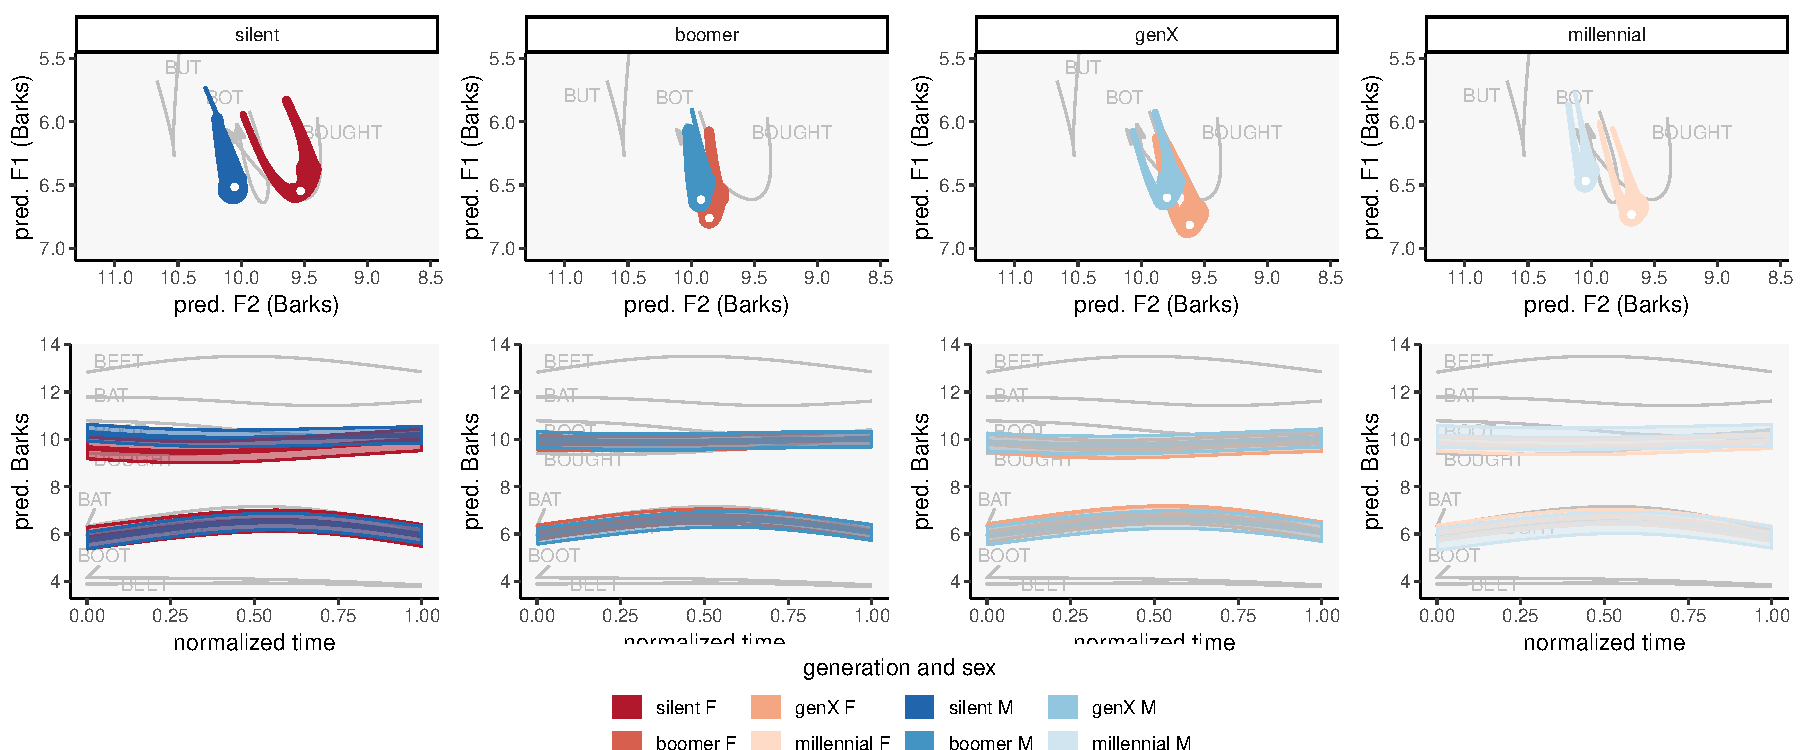
\includegraphics[angle = 90, origin = c, height = \textwidth]{Figures/BOT/BOT_sex_panel_plot_wide.pdf}
	\caption[Predicted formant measurements for \lot by generation.]{Predicted formant measurements for \lot by generation.}
	\label{fig:BOT_sex_panel_plot_wide}
\end{figure*}

Finally, Figure \ref{fig:BOT_sex_panel_plot_wide} compares the two sexes' \lot trajectories. All four plots suggest that the women's realizations of \lot are further back than the men's, by varying degrees. In the Silent generation, this difference in F2 was significant for 90\% of the duration of the vowel (\ref{fig:bot_diff_smooths_sex_gen}B). But, in the middle two generations, there was no difference (\ref{fig:bot_diff_smooths_sex_gen}C--F), and looking back at Figure \ref{fig:BOT_four_panel}, this lack of significance is a result of the two sexes converging somewhere in the middle of the F2 gap that separated the sexes in the Silent generation.

However, a cursory look at the Millennials may suggest that \lot-retraction has begun. Among the Millennials, the women generally used a variant of \lot that was statistically both more retracted and lower than the men (\ref{fig:bot_diff_smooths_sex_gen}G--H). On the one hand, this retraction is in line what what would be expected in a western community, and is an indication that this shift has spread into Cowlitz County. On the other hand, the lowering is opposite of the expected pattern. As it turns out, this difference is primarily an effect of the men using a more fronted and raised variant than the women lowering and retracting (cf. Figure \ref{fig:BOT_four_panel}). Therefore, I cannot conclude that even the Millennial women, who are typically the most conservative, are shifting \lot.

Concluding this section on \lot, there is no evidence of any meaningful change in this vowel. Comparing generations and sexes, we see raising, lowering, retraction, and advancement all happening in the vowel space, not to mention slight changes in trajectory shape. There were no consistent changes that spanned multiple generations, and the patterns that did reach significance were not always in the expected direction of change.




\section{\thought}
\label{BOUGHT}

In this sample, there were 3,819 tokens of \thought coming from 311 unique words. The most common of these words were \textit{long}, \textit{Longview}, \textit{thought}, \textit{talk(ing)}, \textit{bought}, \textit{across}, \textit{water}, \textit{Washington}, \textit{gone}, and \textit{watch}. There was an average of 71 tokens per speaker\footnote{Speakers ranged from 24 to 210 tokens with a standard deviation of 31.7: 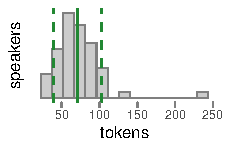
\includegraphics[width = 1.5in]{Figures/BOUGHT/BOUGHT_tiny.pdf}} and 477 tokens from each sex within each generation.

%\begin{figure}[htb]
%	\centering
%	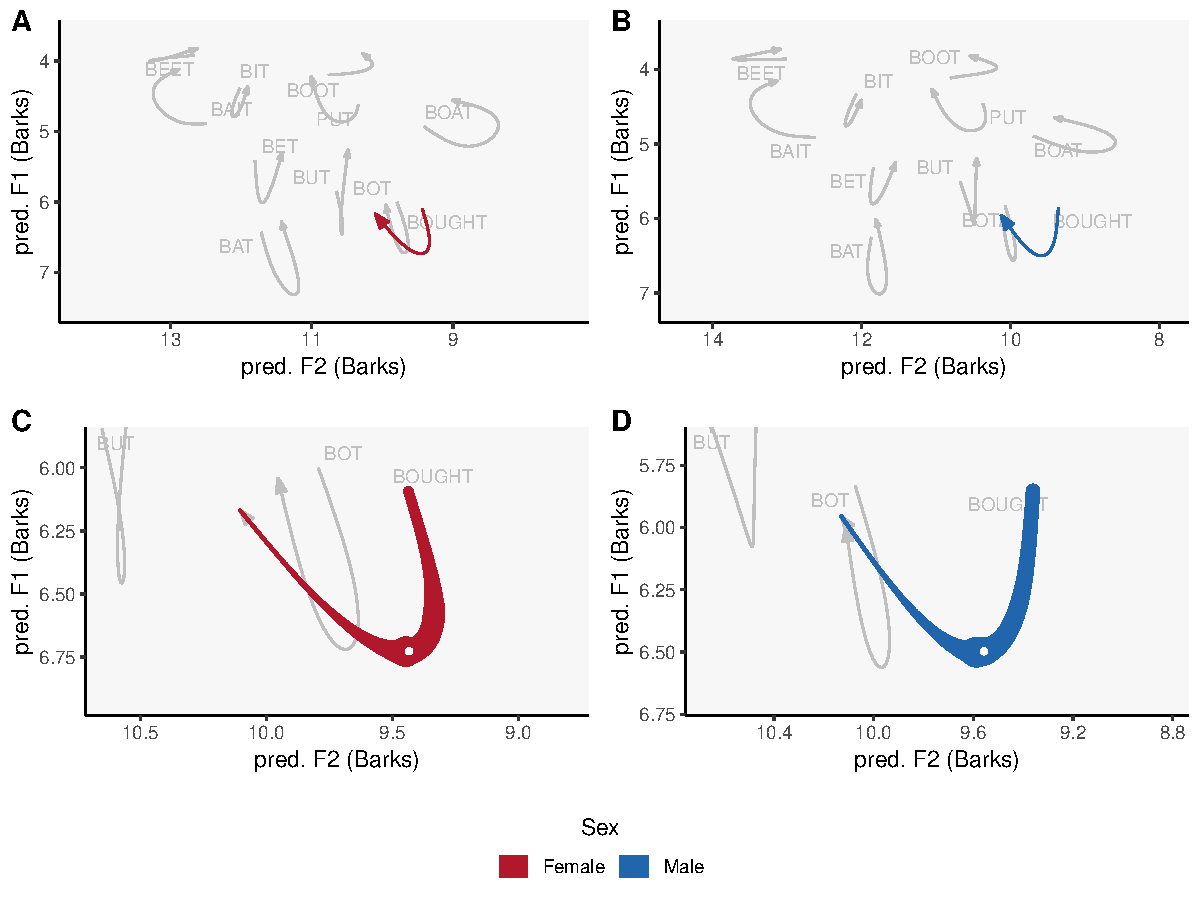
\includegraphics[width = \textwidth]{Figures/BOUGHT/BOUGHT_four_panel_plot_summarized.pdf}
%	\caption[Predicted formant measurements for \thought by sex.]{Predicted formant measurements for \thought by sex with women on the left and men on the right. Predicted values are averaged across all generations.}
%	\label{fig:BOUGHT_four_panel_summarized}
%\end{figure}

%To get an overall look at the

\begin{figure*}[tb!]
	\centering
	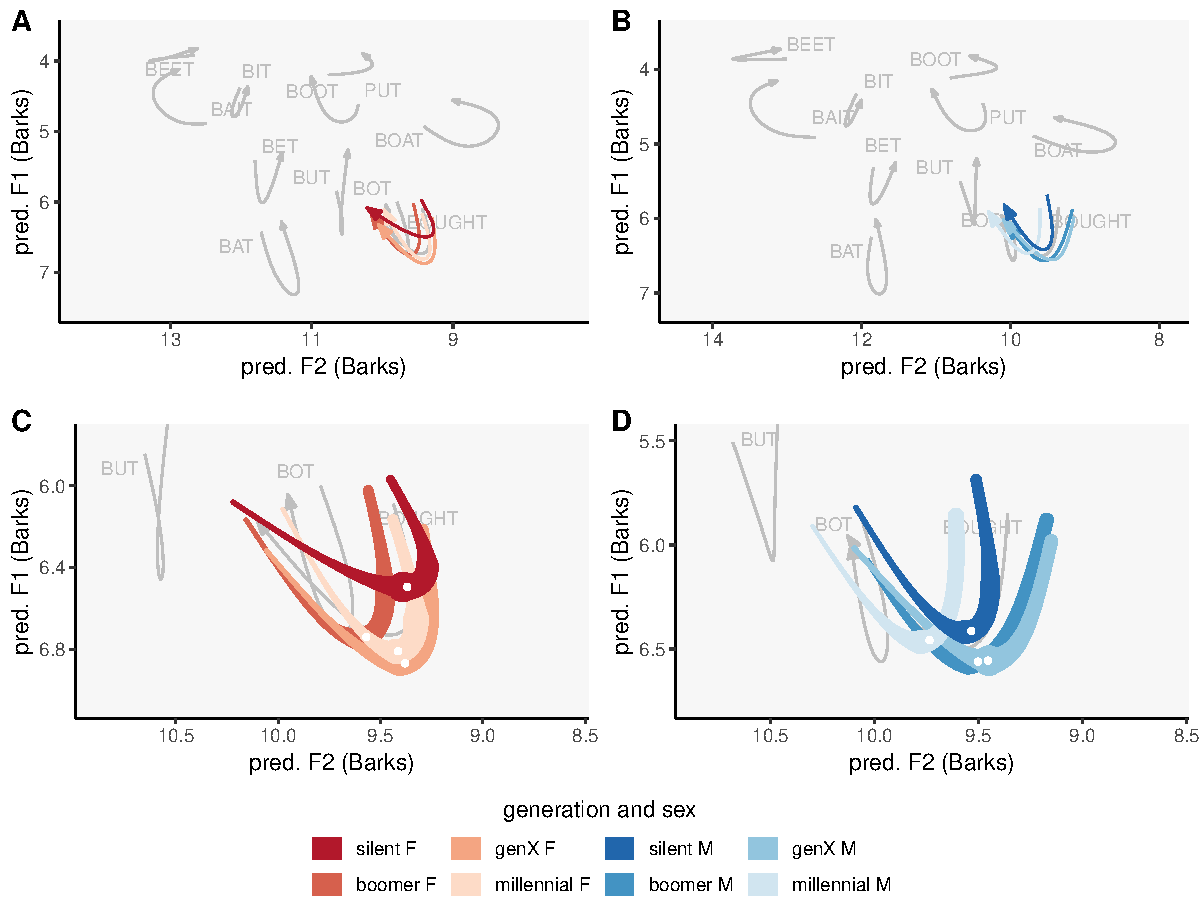
\includegraphics[width = 6.5in]{Figures/BOUGHT/BOUGHT_four_panel_plot.pdf}
	\caption[Predicted formant measurements for \thought by sex and generation.]{Predicted formant measurements for \thought by sex and generation. Women are on the left and men on the right. Darker shades represent older generations.}
	\label{fig:BOUGHT_four_panel}
\end{figure*}

Figure \ref{fig:BOUGHT_four_panel} presents a view of how \thought has changed in apparent time between the two sexes. Like \lot, we see here that the differences between generations are again relatively small, especially in panels A and B which show the change in the context of the full vowel space. Beginning with the women, the direction of shifting bears a resemblance with the patterns in \lot: the Silent generation uses the highest and backest variant, the Baby Boomers use the frontest, and there is little difference between the youngest two generations, which are somewhere in the middle. The difference smooths confirm that Generation X and the Millennials are significantly lower than the Silent Generation (\ref{fig:bought_diff_smooths_gen}E,I). Among the men, we again see inconsistent shifting, with the Silent generation using the highest vowels and the Millennials the frontest, but overall amount of shift in the F1-F2 space is small. Difference smooths suggest some significance in the vowels, chiefly showing that the middle two generations have lower and backer vowel onsets (\ref{fig:bought_diff_smooths_gen}, right two columns). The pattern found in both sexes is some lowering, fronting, and backing, but not the expected raising that found in the merged low back vowel in other western communities.

\begin{figure*}[p]
	\centering
	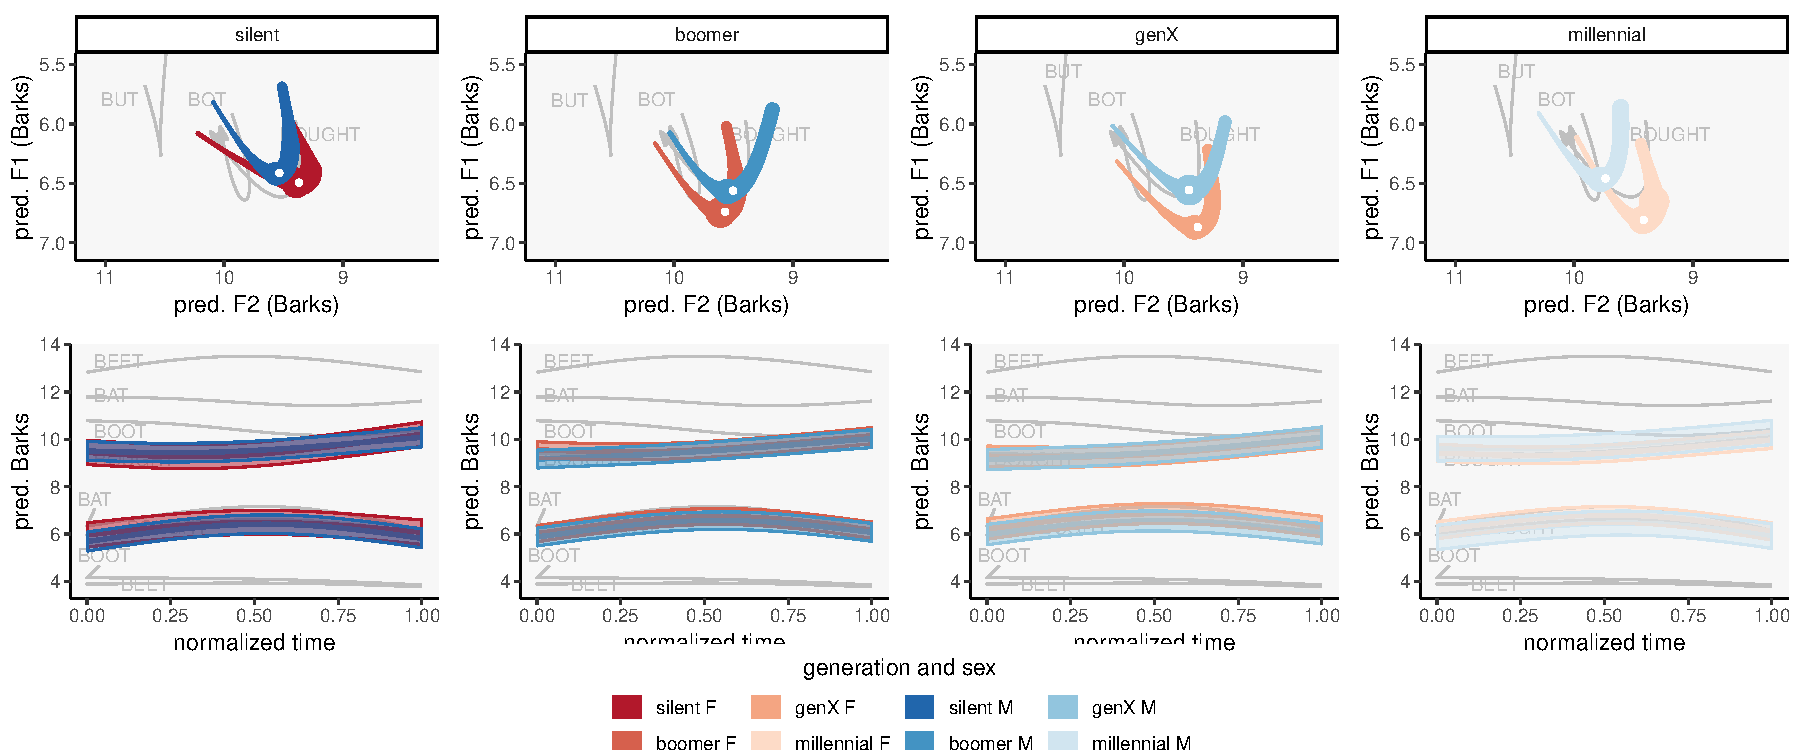
\includegraphics[angle = 90, origin = c, height = \textwidth]{Figures/BOUGHT/BOUGHT_sex_panel_plot_wide.pdf}
	\caption[Predicted formant measurements for \thought by generation.]{Predicted formant measurements for \thought by generation.}
	\label{fig:BOUGHT_sex_panel_plot_wide}
\end{figure*}

Finally, Figure \ref{fig:BOUGHT_sex_panel_plot_wide} compares the two sexes' realizations of \thought across generations. Generally, we see that women tend to use lower variants than the men, but whether they are fronter or backer depends on the generation. Difference smooths suggest only a few portions are statistically significant, the largest confirming the vowel height difference in Generation X and the Millennials (\ref{fig:bought_diff_smooths_sex_gen}E,G). Again, if women assumed to be leading language change in this community, the trajectory of shifting would be that of lowering (and possible backing) of \thought, which is an unexpected direction of change.

Summarizing \thought, this section has shown that there is relatively little change in apparent time. Difference smooths indicated that some portions of vowel trajectories were different across generations and between sexes, but, like \lot, there was no consistent direction of shifting. It appears then that \thought is relatively stable in this community and does not participate in the shifting found in other western communities or even other parts of the vowel space in these speakers.

\section{Discussion}

In this chapter, I have provided evidence to reject the hypothesis of a low back merger in Cowlitz County. \lot was significantly fronter than \thought was, particularly at the vowel onset. Difference smooths and visualizations of raw data confirm what is seen in the predicted formant measurements. Furthermore, neither \lot nor \thought show any real indication of shifting in this community. There were some differences across generations and between the sexes, but the shifting was inconsistent across apparent time, and rarely in the direction of expected change. Overall, the differences that exist between social groups are small.

\subsection{Is the low back merger a pan-western feature?}

As the editors of \textit{Speech in the Western States} state, ``the low back merger can certainly be called a pan-Western dialect feature'' \citep[167]{fridland_etal_2017_pads}. Nevertheless, as discussed in \S\ref{position_low_back_vowels}, numerous studies have found that the merger is not complete.

For example, the \textit{Atlas of North American English} reports that San Francisco stands out as a place where \lot and \thought are not (yet) fully merged \citep[64]{labov_ash_boberg_2006_anae}. Other studies \citep{moonwomon_1991_diss, hall_lew_2013} have confirmed this finding, and San Francisco has become known as somewhat of an anomalous city in the West in this regard. However, that same atlas also reports that the front lax vowels were not shifting in the West, but dozens of research papers and presentations have shown otherwise. Labov addressed this discrepancy,\footnote{At the annual meeting of the American Dialect Society in 2018 in Salt Lake City, Kara Becker moderated a panel entitled \textit{Chain shifting in the Third Dialect: A dialogue on the similarities between the California and Canadian Vowel Shifts}; Labov was the discussant at the end of that panel.} stating that the large body of research that has recently come out of the West has demonstrated that there is indeed a lot going on in this region. This research has filled in some of the regional, temporal,\footnote{A few of my youngest participants were not even born when the data for the \textit{Atlas of North American English} was collected. Recently collected data in the West is an entire generation younger than that data from that study.} and methodological gaps that the \textit{Atlas of North American English} could not cover; we have a greater understanding of the speech in this region than could have been reported in a large-scale project.

Now that more focused research has been conducted on various communities across the West, it appears that San Francisco is not unique. Evidence of a contrast between \lot and \thought has been found in Salt Lake City \citep{dipaolo_1992}, Colorado \citep{holland_brandenburg_2017_pads}, Nevada \citep{fridland_kendall_2017_pads}, Portland \citep{becker_etal_2016_pads}, and now Cowlitz County. These are all areas that admittedly realize \lot and \thought very close to each other, but with evidence of separation.

In fact, many of the studies that do test for and confirm the presence of the low back merger do so with relatively simplistic measures. Sometimes, the vowels are considered merged by visual inspection of single-point measurements, sometimes grouped by speaker or social class \citep{brumbaugh_koops_2017_pads, kennedy_grama_2012, wassink_2015}, or by acoustic similarity coupled with speaker intuition \citep[59]{labov_ash_boberg_2006_anae}. In other cases, the vowels were considered merged if \textit{t}-tests on their distributions did not achieve statistical significance \citep{bar_el_etal_2017}.\footnote{With sufficient data, \textit{t}-tests may be a viable (albeit simplistic) method for measuring merger, but when only ``five or six tokens of each low back vowel'' \citep[122]{bar_el_etal_2017} are included in a \textit{t}-test, there is just not enough statistical power to find significance in even between relatively large differences.} It may be the case that when more sophisticated measures of merger are applied in other western communities, a small difference between the vowels may still be found, even when visual inspection says otherwise.

Because of the growing number of studies showing that \lot and \thought are not completely merged, perhaps it would be better to consider the \textit{approximation}\footnote{By \textit{approximation}, I refer to the position of the vowels in the vowel space rather than approximation of the articulators.} of the low back vowels to be a pan-Western feature, rather than the merger itself. When explicitly tested, it appears that a small but significant separation is more common than a full merger. Indeed, inspection of Map 9.2 in the \textit{Atlas of North American English} show that many speakers in the West lack a full merger, and ``transitional'' speakers coexist with fully merged speakers in most western cities (including all areas sampled in the Pacific Northwest).

Finally, it may be the case that this approximation of the low back vowels is stable in the West. In Cowlitz County,there is no evidence of a trend towards merger: the low back vowels are as distinct in the Millennials as they are in the Silent generation.\footnote{For comparability with previous studies, I ran a mixed-effects linear regression model with the \texttt{lmer} function in the \texttt{lme4} package \citep{bates_etal_2015_lme4} with age as a continuous predictor interacted with sex, and speaker and word as random intercepts. The midpoints of each vowel were the dependent variables. No significant effect for age or sex was found for either F1 or F2 for either \lot our \thought.} A similar lack of convergence in apparent time is found in Colorado \citep[18]{holland_brandenburg_2017_pads}, Nevada \citep[148]{fridland_kendall_2017_pads}, and Oregon \citep[115]{becker_etal_2016_pads}. This does not imply that this distinction will be maintained: \citet{herold_1990_diss} and \citet{johnson_2010_pads} both show that gradual demographic shifts can tip the scale at some point, causing a sudden loss in contrast between \lot and \thought. Nevertheless, despite major events in Cowlitz County (the establishment of Long-Bell in the 1920s and the collapse of the timber industry in the late 1970s), this distinction is still maintained in Cowlitz County.

\subsection{Raising of \lot/\thought and the shape of the vowel space}

The other pattern that is found in other western communities is that the merged low back vowel, or sometimes the the nearly merged pair \citep[19]{holland_brandenburg_2017_pads} is backing and possibly also raising. In Cowlitz County, there was no evidence of such a pattern. Both \lot and \thought are remarkably stable in apparent time.

The raising of the merged vowel has implications for the shape of the vowel space in other Third Dialect areas. In California \citep[23--24]{donofrio_etal_2017_pads} and in Canada \citep{boberg_2011}, this raised vowel, together with the retraction of \trap, causes a triangular vowel space rather than the prototypical trapezoidal one described for American English with its two low vowels. In Cowlitz County, the shape of the vowel space can still generally be described as trapezoidal. For the majority of speakers, \trap is the lowest vowel, but because \thought is firmly low, it forms a distinct second low corner.

In \S\ref{sec:geography_of_elsewhere_shift}, I point out that Washington is positioned between two areas that are known for their innovative realizations of the Elsewhere Shift: California and Oregon to the south and British Columbia to the north. Other researchers have commented on the lack of Washingtonians that exhibit the lowered or retracted \bat, \bet, and \bit. In this study, I have shown that at least in Cowlitz County there are speakers with this shift. Nevertheless, it appears that even southwest Washington has resisted the raising of the low back vowels.



\subsection{Structural relationship with other vowels}

In \S\ref{sec:relationship_between_front_lax_vowels}, I explain that there are mixed reports regarding whether the low back merger is structurally related to the lowering of front lax vowels. Numerous researchers have stated that the low back merger is the trigger that caused \trap to retract (e.g. \citealt[212]{clarke_etal_1995}, \citealt[139]{gordon_2006}, and \citealt[220]{labov_ash_boberg_2006_anae}). Nevertheless, there have been others who have expressed doubts that the two are related. In Kansas City, \citeauthor{strelluf_2019} finds younger speakers have \trap further along the front diagonal than older speakers, but that people of all ages had a high degree of overlap between \lot and \thought: ``[f]or the Kansas Citians in this sample, \lot and \thought overlap phonetically and \trap retracts, but one sound change does not appear to depend on the other'' \citeyearpar[76]{strelluf_2019}. Just as has been found in California \citep{kennedy_grama_2012}, Colorado \citep{holland_2014_diss}, and Illinois \citep{bigham_2010}, speakers in Cowlitz County appear to have shifted \trap without shifting \lot (or \thought).

In that case, what is the trigger then for the Elsewhere Shift? To answer this question, it may be helpful to review the timeline of the changes found with the front lax vowels. In \S\ref{sec:what_kind_of_shift}, I hypothesize that \bat began shifting one generation before the Silent Generation, so around the 1920s or 1930s (concurrently with the establishment of Longview in 1923). \bet began lowering approximately between the 1940s and 1950s, with \bit beginning to shift around the late 1970s or early 1980s (concurrently with the fall of the timber industry).

For \lot and \thought, the vowels have been stable for at least the four generations in this sample. Rather than positing no change whatsoever, it may be the case that the convergence of \lot and \thought had already reached completion by the time the Silent Generation acquired language and that this near merger has been stable for the past 80 years. This is supported by early reports from the Pacific Northwest: the two low back vowels are described as being indistinguishable in mid-century Washington English, particularly in the western half of the state \citep{reed_1952}. Massive changes in the demographics of an area can lead to merger, such as the influx of Eastern European settlers into Western Pennsylvania \citep{herold_1990_diss}, the expansion of Kansas City as people came to the cities from the rural areas in search of jobs after the Great Depression \citep{strelluf_2019}, or a gradual population shift from near Boston to western Connecticut \citep{johnson_2010_pads}. As explained in \S\ref{sec:longview_a_planned_city}, Cowlitz County was settled by a diverse population. Like many other areas of the West, this mixture of speech varieties may have been the trigger for \lot retracting towards \thought, just as it was in other areas of the United States. As Longview exploded into existence, newcomers adopted the nearly-merged low back vowels by means of the Founder Principle, resulting in a stable approximation of the two vowels by the time the Silent Generation acquired language. This scenario is plausible given the history of the area and patterns found in other areas, but it remains speculative because data before the Silent Generation has not yet been analyzed.

The point is that these two vowels have been stable for some time. But theoretically they were not always to close because the canonically front vowel, \lot, is no longer front. Regardless of how the two vowels approached each other, it appears that that sound change antedates when \trap began shifting and may in fact be related to the shifting of the front lax vowels. But rather than their merging that was the trigger---because the two vowels are not merged in this community---it is their approximation that set \bat into motion. I therefore conclude that, at least in this sample of Cowlitz County residents, the low back and the front lax vowels are structurally related.

Given this finding, the relationship between the shifting vowels in the Elsewhere Shift and their relative timing is still variable across communities. In addition to the low back vowels acting as the trigger as I have found here, some have found that it was \bat that began shifting \citep{kennedy_grama_2012, becker_etal_2016_pads} or even \dress \citep{holland_2014_diss}. And then there are accounts of all vowels shifting at once \citep{boberg_2005, lawrance_2002_thesis, donofrio_etal_2019} or haphazardly with no pattern \citep{pratt_etal_2018}. Clearly there is not a unified description of this shifting in regions with the Elsewhere Shift. It actually appears that communities generally converge on similar eventual results, but as far as \textit{how} they do so depends on other factors. In fact, \citet[23--25]{donofrio_etal_2017_pads} explicitly describe this two-pronged approach in California in relation to the eventual position of the merged low back vowel: in Redding the low back vowels merged by moving closer together before raising while in Merced and Bakersfield \thought was stable in the higher position and \lot raised to meet it. If different communities can shift along different paths to eventually reach the same target, we may be finding widespread variation in the West and Canada regarding the \textit{process} of the Elsewhere Shift. This begs the next question of why they do converge on the same result. I add my voice to the chorus of other scholars who have said the same thing: more work is required---on their formant dynamics, on perception of the two vowels, on more communities in the West, and on legacy data from before the Silent Generation---to fully understand the Elsewhere Shift, including the low back merger.

\subsection{The use of GAMMs in the low back merger}

I close this section with yet another justification for the use of GAMMs to study merger and what insight can be gained that could not have been found otherwise.

Just as was found with all other vowels, studying vowel dynamics illuminated more detail about how the low back vowels are realized. A single-point analysis on vowel midpoints would have concluded that \lot and \thought are merged, and that this difference is stable across time. Nevertheless, the vowels not only differ in their relative position but also in their dynamics, with \thought continuing to be a more dynamic vowel like it is in other parts of the country. Difference smooths revealed that the two vowels differ primarily in their onset rather than their offset.

In addition to the predicted values, analyzing vowel trajectories is useful when examining vowel plots of raw data. Figure \ref{fig:jessica_low_back} shows that Jessica's two vowels have nearly identical midpoints, leading a single-point analysis to show that she is merged. When the full trajectory is considered though, it becomes clear that she does differentiate between the vowels by using rising F2 over the course of \thought but not for \lot.

In general, the informed use of GAMMs to study vowel merger is a fruitful method of research. They take into account more information from the acoustic signal than single-point measurements alone, meaning their results should match human perception better. \citet{dipaolo_faber_1990} show that vowels can be distinct even when their midpoints overlap, and that that voice quality can be the differentiating factor. With the adoption of GAMMs and other techniques to study vowel merger, we may find other properties of a vowel---like its trajectory---that keep it distinct from another.\footnote{After all, \price and \mouth are not merged even though their nuclei are very close for many speakers.} This additional insight into how vowels are realized may further our understanding of exceptional cases like near-mergers and flip-flops \citep{hall_lew_2013}, which are problematic in our current theory of sound change.

\section{Conclusion}

In this chapter, I have shown that the low back vowels are not merged in Cowlitz County. \lot was significantly more fronted and \thought had a more dynamic trajectory. Furthermore, this pattern was stable in apparent time. I suggest that \lot approximated \thought's position in the vowel space before the 1930s in Cowlitz County as a result of a mixture of dialects spoken in the area; this, in turn, acted as the for \trap shifting. I call for additional research on the low back vowels and its relationship to the Elsewhere Shift and suggest that a bona fide merger may not be as widespread as previously reported. The use of dynamic modeling can help further our understanding of these vowels and mergers more generally.
